\documentclass[border=6pt]{standalone}
\usepackage{tikz}
\usepackage{pgfplots}
\pgfplotsset{compat=1.18}
\usetikzlibrary{arrows.meta,positioning,shapes.geometric,fit,backgrounds,calc,decorations.pathreplacing,patterns,pgfplots.groupplots}
\tikzset{
  blk/.style={rectangle, rounded corners=2pt, draw=black!70, thick, fill=blue!6,
              minimum height=8mm, minimum width=20mm, align=center, font=\small},
  io/.style={rectangle, rounded corners=6pt, draw=black!70, thick, fill=green!8,
             minimum height=8mm, align=center, font=\small},
  proc/.style={rectangle, draw=black!70, thick, fill=orange!10, minimum height=8mm,
               align=center, font=\small},
  dec/.style={diamond, aspect=2, draw=black!70, thick, fill=yellow!15, align=center, font=\footnotesize},
  warnbox/.style={rectangle, rounded corners=2pt, draw=red!60!black, thick, fill=red!7,
                  minimum height=8mm, align=center, font=\small},
  oklbox/.style={rectangle, rounded corners=2pt, draw=green!45!black, thick, fill=green!8,
                 minimum height=8mm, align=center, font=\small},
  ar/.style={-{Latex[length=2mm]}, thick},
  arl/.style={-{Latex[length=2mm]}, thick, dashed, draw=black!55},
  lbl/.style={font=\footnotesize\itshape, text=black!60},
}
\definecolor{good}{RGB}{34,139,34}
\definecolor{bad}{RGB}{178,34,34}
\definecolor{warn}{RGB}{218,165,32}
\definecolor{pesblue}{RGB}{0,45,98}
\definecolor{complete}{RGB}{30,125,79}
\definecolor{partial}{RGB}{176,106,0}
\definecolor{blocked}{RGB}{166,43,43}
\newcommand{\gl}[1]{{\tiny\color{black!75}#1}}
% --- figure-local styles -------------------------------------------------
\tikzset{
  q/.style={dec, minimum width=6.20cm, minimum height=2.60cm, text width=3.30cm,
            inner sep=2pt},
  leaf/.style={rectangle, rounded corners=2pt, thick, draw=black!70, fill=white,
               text width=3.55cm, minimum height=2.60cm, inner sep=3pt,
               align=center, anchor=north, font=\scriptsize},
  leafc/.style={leaf, draw=complete!75!black, fill=complete!8},
  leafp/.style={leaf, draw=partial!75!black, fill=partial!8},
  leafb/.style={leaf, draw=blocked!75!black, fill=blocked!8},
  root/.style={blk, text width=8.00cm, inner sep=4pt},
  countb/.style={oklbox, text width=3.55cm, inner sep=3pt, font=\scriptsize,
                 align=center, anchor=north},
  sw/.style={draw=black!70, thick, minimum width=3.4mm, minimum height=3.4mm,
             inner sep=0pt},
  swl/.style={font=\scriptsize, anchor=west, text=black!80},
  st/.style={font=\scriptsize\bfseries},
  gl/.style={font=\tiny, align=center, text=black!75},
  yesno/.style={lbl, fill=white, inner sep=1pt, font=\scriptsize},
}
\begin{document}
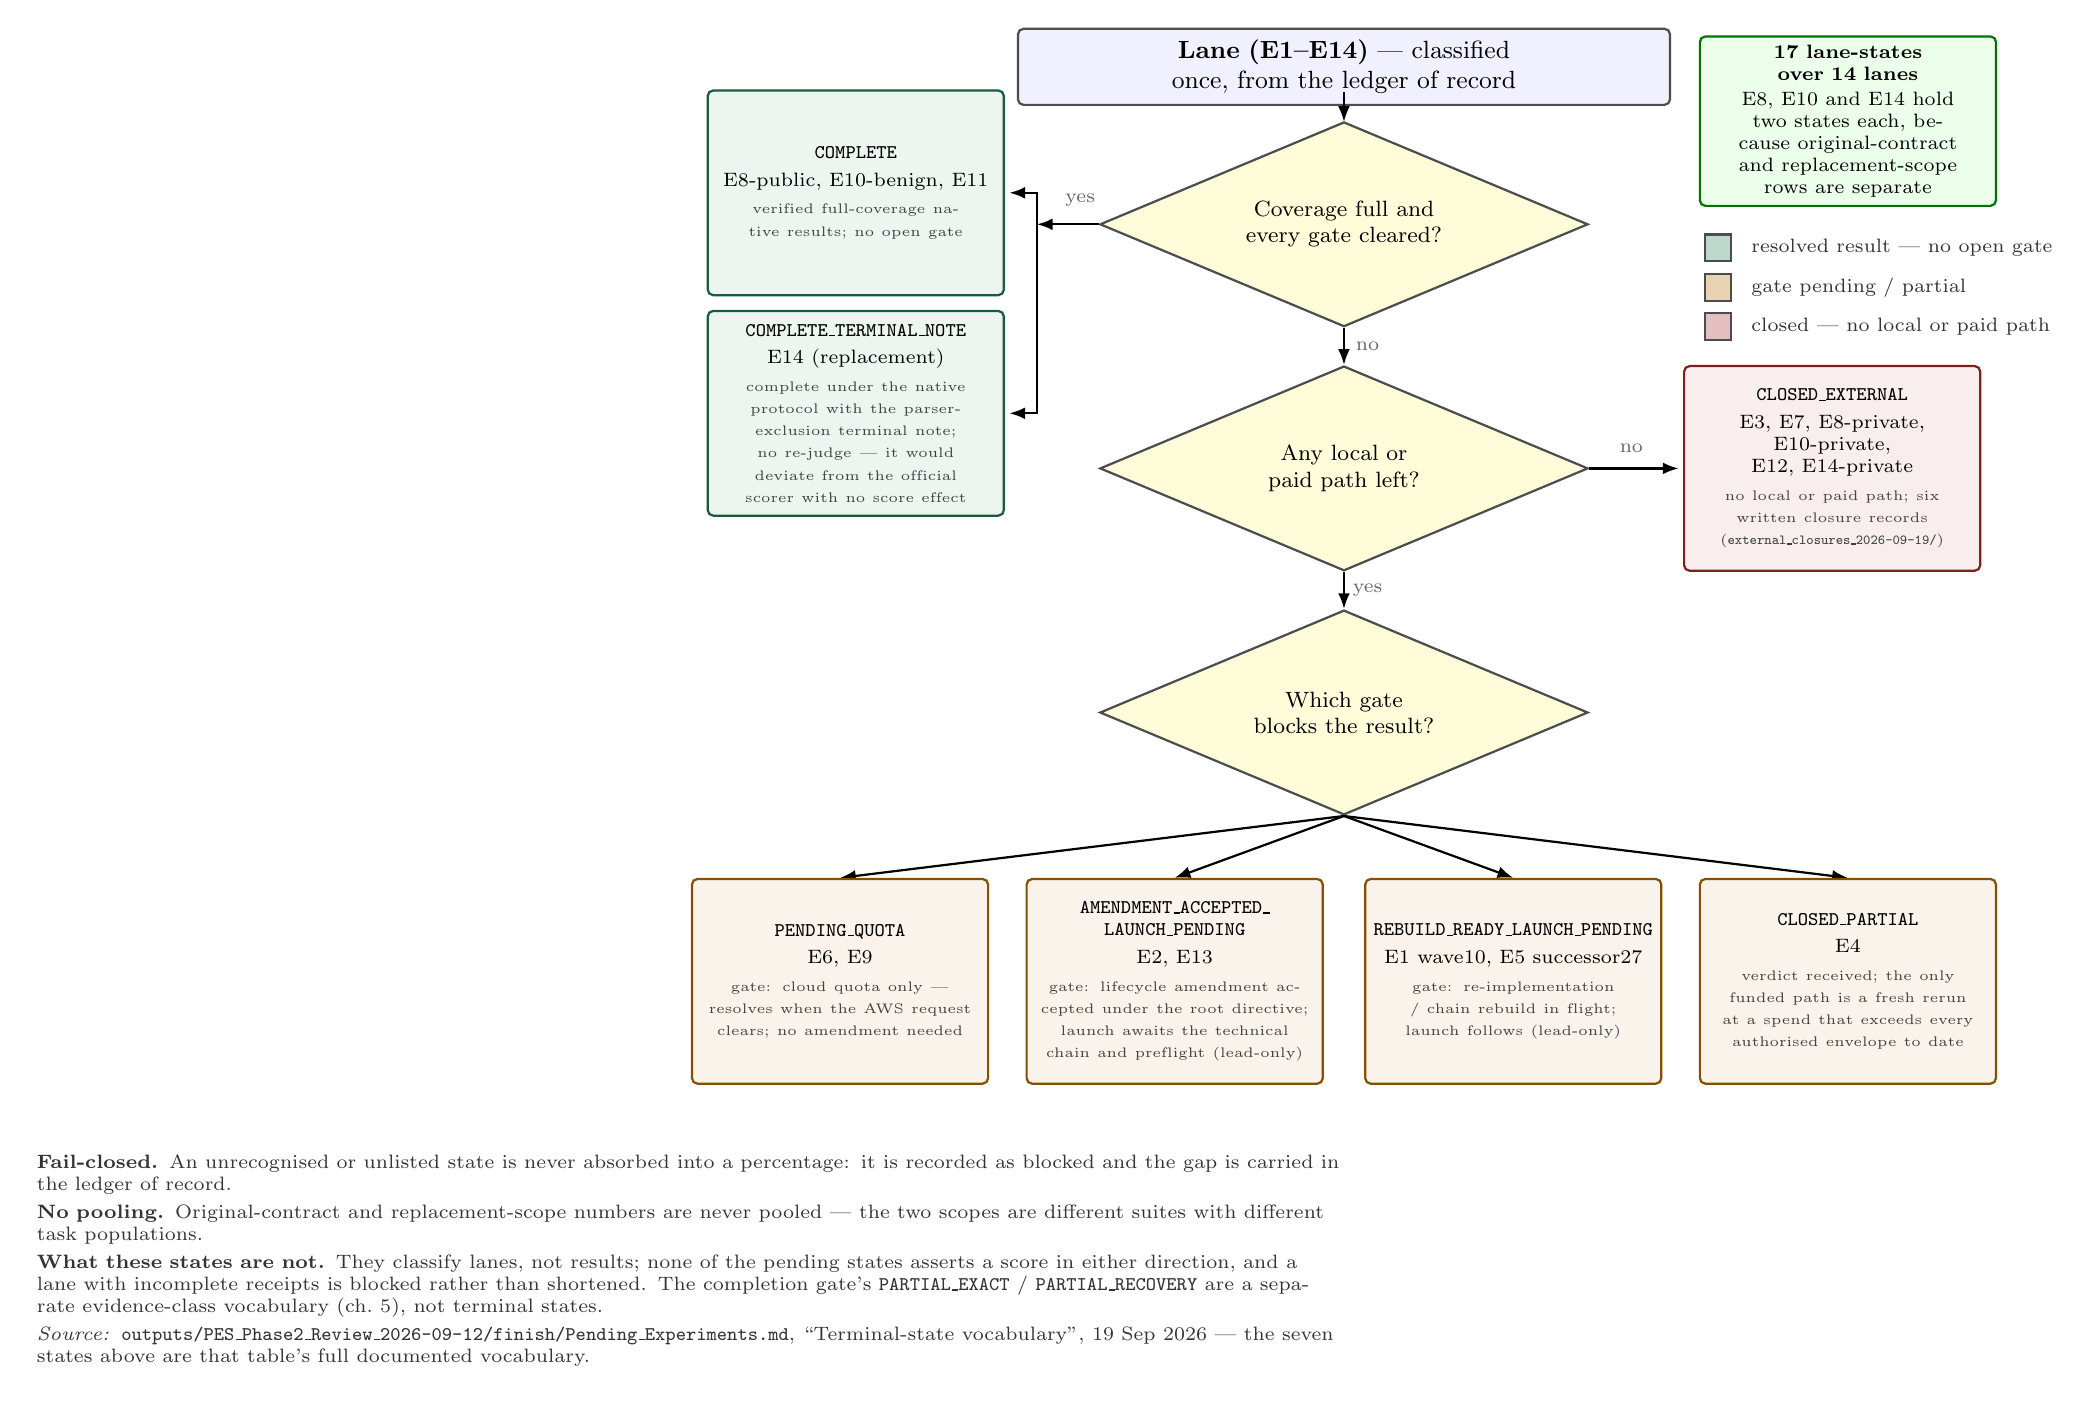
\begin{tikzpicture}[x=1cm,y=1cm]

% ===================== ROOT =====================
\node[root] (ROOT) at (0,0)
  {\textbf{Lane (E1--E14)} --- classified once, from the ledger of record};
\draw[ar] (0,-0.32) -- (0,-0.70);

% ===================== legend (top right) =====================
\node[countb] (CNT) at (6.40,0.40)
  {\textbf{17 lane-states over 14 lanes}\\[1pt]
   E8, E10 and E14 hold two states each, because original-contract and
   replacement-scope rows are separate};
\node[sw, fill=complete!30]           at (4.75,-2.30) {};
\node[swl] at (5.05,-2.30) {resolved result --- no open gate};
\node[sw, fill=partial!30]            at (4.75,-2.80) {};
\node[swl] at (5.05,-2.80) {gate pending / partial};
\node[sw, fill=blocked!30]            at (4.75,-3.30) {};
\node[swl] at (5.05,-3.30) {closed --- no local or paid path};

% ===================== Q1 =====================
\node[q] (D1) at (0,-2.00) {Coverage full and every gate cleared?};
\node[q] (D2) at (0,-5.10) {Any local or paid path left?};
\node[q] (D3) at (0,-8.20) {Which gate blocks the result?};

% Q1 yes -> two leaves on the left
\draw[ar] (D1.west) -- (-3.90,-2.00);
\draw[ar] (-3.90,-2.00) -- (-3.90,-1.60) -- (-4.25,-1.60);
\draw[ar] (-3.90,-2.00) -- (-3.90,-4.40) -- (-4.25,-4.40);
\node[yesno] at (-3.35,-1.70) {yes};

\node[leafc, anchor=center] (L1) at (-6.20,-1.60)
  {\textbf{\texttt{COMPLETE}}\\[2pt]
   E8-public, E10-benign, E11\\[2pt]
   \gl{verified full-coverage native results; no open gate}};
\node[leafc, anchor=center] (L2) at (-6.20,-4.40)
  {\textbf{\texttt{COMPLETE\_}\allowbreak\texttt{TERMINAL\_NOTE}}\\[2pt]
   E14 (replacement)\\[2pt]
   \gl{complete under the native protocol with the parser-exclusion terminal
   note; no re-judge --- it would deviate from the official scorer with no
   score effect}};

% Q1 no -> Q2
\draw[ar] (D1.south) -- (D2.north);
\node[yesno] at (0.30,-3.55) {no};

% ===================== Q2 =====================

% Q2 no -> CLOSED_EXTERNAL
\draw[ar] (D2.east) -- (4.25,-5.10);
\node[yesno] at (3.65,-4.85) {no};
\node[leafb, anchor=center] (L3) at (6.20,-5.10)
  {\textbf{\texttt{CLOSED\_}\allowbreak\texttt{EXTERNAL}}\\[2pt]
   E3, E7, E8-private,\\ E10-private, E12, E14-private\\[2pt]
   \gl{no local or paid path; six written closure records
   (\texttt{external\_clos}\allowbreak\texttt{ures\_2026-09-19/})}};

% Q2 yes -> Q3
\draw[ar] (D2.south) -- (D3.north);
\node[yesno] at (0.30,-6.65) {yes};

% ===================== Q3 =====================

% Q3 -> four leaves
\foreach \x in {-6.40,-2.15,2.15,6.40}
  \draw[ar] (D3.south) -- (\x,-10.30);

\node[leafp] (L4) at (-6.40,-10.30)
  {\textbf{\texttt{PENDING\_QUOTA}}\\[2pt]
   E6, E9\\[2pt]
   \gl{gate: cloud quota only --- resolves when the AWS request clears; no
   amendment needed}};
\node[leafp] (L5) at (-2.15,-10.30)
  {\textbf{\texttt{AMENDMENT\_}\allowbreak\texttt{ACCEPTED\_}\allowbreak\texttt{LAUNCH\_}\allowbreak\texttt{PENDING}}\\[2pt]
   E2, E13\\[2pt]
   \gl{gate: lifecycle amendment accepted under the root directive; launch
   awaits the technical chain and preflight (lead-only)}};
\node[leafp] (L6) at (2.15,-10.30)
  {\textbf{\texttt{REBUILD\_}\allowbreak\texttt{READY\_}\allowbreak\texttt{LAUNCH\_}\allowbreak\texttt{PENDING}}\\[2pt]
   E1 wave10, E5 successor27\\[2pt]
   \gl{gate: re-implementation / chain rebuild in flight; launch follows
   (lead-only)}};
\node[leafp] (L7) at (6.40,-10.30)
  {\textbf{\texttt{CLOSED\_PARTIAL}}\\[2pt]
   E4\\[2pt]
   \gl{verdict received; the only funded path is a fresh rerun at a spend that
   exceeds every authorised envelope to date}};

% ===================== FOOTNOTES =====================
\emergencystretch=1em
\node[anchor=north, align=left, text width=16.60cm, font=\scriptsize, text=black!80]
  at (-8.30,-13.70)
  {\textbf{Fail-closed.} An unrecognised or unlisted state is never absorbed
   into a percentage: it is recorded as blocked and the gap is carried in the
   ledger of record.\\[2pt]
   \textbf{No pooling.} Original-contract and replacement-scope numbers are
   never pooled --- the two scopes are different suites with different task
   populations.\\[2pt]
   \textbf{What these states are not.} They classify lanes, not results; none
   of the pending states asserts a score in either direction, and a lane with
   incomplete receipts is blocked rather than shortened. The completion gate's
   \texttt{PARTIAL\_EXACT} / \texttt{PARTIAL\_RECOVERY} are a separate
   evidence-class vocabulary (ch.~5), not terminal states.\\[2pt]
   {\itshape Source:} \texttt{outputs/PES\_Phase2\_Review\_2026-09-12/finish/}\allowbreak\texttt{Pending\_Experiments.md},
   ``Terminal-state vocabulary'', 19 Sep 2026 --- the seven states above are
   that table's full documented vocabulary.};

\end{tikzpicture}
\end{document}
